\documentclass[uplatex, a4paper, dvipdfmx, 12pt]{jsreport}

\usepackage{jvlisting, listings} %日本語のコメントアウトをする場合jvlisting(もしくはjlisting)が必要
	%ここからソースコードの表示に関する設定
	\lstset{
		basicstyle={\ttfamily},
		frame = trbl, % 上下に線
		tabsize = 2, % タブはスペース2個分に変換
		breaklines=true, % 行が長い場合に折り返す
		columns=[l]{fullflexible}, % 列幅を自動調整する(見た目が良くなる)
	}
	% https://zenn.dev/niyaton/articles/9fa4daaab48d16
\usepackage{docmute}
%このファイルではプリアンブル部分をまとめて書いている
%texworks -stylesheet .\texlive\2022\bin\win32\user.cssは、texの文字だか背景だかを変化させるファイル
\usepackage[dvipdfmx]{graphicx,xcolor}

\usepackage[export]{adjustbox} % includegraphicsなどでmax/min width/heightを使えるようにする
% dvipdfmxは日本語のときのみかく
\usepackage{amsmath, amssymb, amsfonts, mathtools} % おまじない

\usepackage[top=20truemm,bottom=20truemm,left=25truemm,right=20truemm, includeheadfoot, dvipdfmx]{geometry} % 余白の設定 includeheadfootでヘッダー、フッターを含めて空白を開ける 恐らくfancyhdrよりも前にする必要がある

\usepackage{braket, derivative} % braket, 微分
\usepackage{physics2} % physicsの代わり
	\usephysicsmodule{ab, doubleprod, diagmat, xmat}
	\renewcommand{\Re}{\operatorname{Re}}
	\renewcommand{\Im}{\operatorname{Im}}
	\newcommand{\Tr}{\operatorname{Tr}}
	\newcommand{\rank}{\operatorname{rank}}
	\newcommand{\order}{\mathcal{O}}

% \usepackage{mathcomp} % 単位 physicsを使う場合はmathcomp
\usepackage{siunitx} % 単位 physicsを使う場合はqtyが衝突するので使わない
\usepackage[version=4]{mhchem} % 化学式

\setcounter{tocdepth}{2} % 目次の深さ
\usepackage[dvipdfmx]{hyperref} % リンク付きref
\usepackage{pxjahyper} % 日本語refの文字化け防止 (u)pLaTexのみ
	\hypersetup{%
		%  dvipdfmx,
		setpagesize=false,%
		bookmarks=true,%
		bookmarksdepth=tocdepth,%
		bookmarksnumbered=true,%
		%  allcolors=blue,%
		hidelinks,
		pdftitle={タイトル},
		pdfauthor={著者の名前},
	}

\usepackage{nameref} % 章の名前を参照
% \usepackage{wtref} % refコマンドを増やす
	% \newref{sec, eq}
	% \newref[scope=chapter]{fig, tb}
	% \setrefstyle{eq}{refcmd=(\ref{#1})}
	% \setrefstyle{sec}{prefix=第, suffx=章}
\usepackage{zref-xr} % ファイルをまたいだref。ref系のパッケージの最後に読み込む
	\zxrsetup{toltxlabel}

\usepackage{ascmac} % 枠
\usepackage{bm} % 太字

\usepackage{here} % 図表の位置
\usepackage{enumitem} % リスト
\usepackage{multirow} % 表で複数マスにまたがるもの
% \usepackage{tikz} % tikz pgfplotsを読み込むと自動で読み込まれるっぽい
% \usetikzlibrary{calc}
\usepackage{pgfplotstable, pgfplots} % 表, グラフ
	\pgfplotsset{
		compat=1.18,
		table/col sep=comma
	}
	\usetikzlibrary{calc}
\usepackage{csvsimple} % csv読み込み
\usepackage[]{caption} % キャプション
\usepackage[subrefformat=parens]{subcaption} % subキャプション
	\captionsetup{compatibility=false}

% \usepackage[compress=false]{graphicscache} % 画像のキャッシュ(動いてない)
\usepackage{fancyhdr} % ヘッダー
	\pagestyle{fancy}
	\lhead{\leftmark} %ヘッダ左
	\chead{} %ヘッダ中央
	\rhead{\rightmark} %ヘッダ右.コンパイルした日付を表示
	\renewcommand{\chaptermark}[1]{\markboth{第\ \normalfont\thechapter\ 章~#1}{}}
	%\renewcommand{\sectionmark}[1]{\markright{\thesection #1}{}}
	\lfoot{} %フッタ左
	\cfoot{\thepage} %フッタ中央.ページ番号を表示
	\rfoot{} %フッタ右
	% \renewcommand{\headrulewidth}{} %ヘッダの罫線
	% \renewcommand{\footrulewidth}{} %フッタの罫線

\usepackage{environ, ifthen, xparse, comment} % 環境の定義, if文, コマンド定義, コメントアウト
% \usepackage{dirtree} % ディレクトリツリー

\usepackage[deluxe]{otf} % utf入力 pxchfonの設定によっては必須
\usepackage[ipaex]{pxchfon} % フォント埋め込み(文字化け防止)
% \usepackage[english, japanese]{babel}
\usepackage[style=phys, articletitle=false, biblabel=brackets, chaptertitle=false, pageranges=false]{biblatex} % bib
	% https://qiita.com/shiro_takeda/items/fac1351495f32c224a28
	% \renewbibmacro{in:}{} % in: Some journal の "in:" を取る
	% https://paper3510mm.github.io/latex/biblatex.html
	\addbibresource{../bib/refs.bib}
	\ExecuteBibliographyOptions{
		sortcites=true,
		% backref=true,
		date=year
	}

	% 日本語文章への対応
	% 下記参考資料ではlangidにenglishなどjapanese以外がある場合はエラーを吐くため、japaneseのみに反応するようにしてenglishがあっても大丈夫なようにしている。
	% http://granular.blog39.fc2.com/blog-entry-76.html
	% https://tex.stackexchange.com/questions/498682/disabling-the-printing-of-language-only-while-using-the-macro-based-on-language
	\newbibmacro*{finalnamedelim:japanese}{\multinamedelim}

	\renewcommand*{\finalnamedelim}{%
		\iffieldequalstr{langid}{japanese}
		{\usebibmacro*{finalnamedelim:\strfield{langid}}}
		{\ifnumgreater{\value{liststop}}{2}{\finalandcomma}{}%
			\addspace\bibstring{and}\space}}

	\newbibmacro*{name:given-family:japanese}[4]{%
		\usebibmacro{name:delim}{#1#2}%
		\usebibmacro{name:hook}{#1#2}%
		#1\bibnamedelimc#2}

	\DeclareNameFormat{given-family}{%
		\iffieldequalstr{langid}{japanese}
		{\usebibmacro*{name:given-family:\strfield{langid}}
			{\namepartfamily}
			{\namepartgiven}
			{\namepartprefix}
			{\namepartsuffix}}%
		{\ifgiveninits
			{\usebibmacro{name:given-family}
				{\namepartfamily}
				{\namepartgiveni}
				{\namepartprefix}
				{\namepartsuffix}}
			{\usebibmacro{name:given-family}
				{\namepartfamily}
				{\namepartgiven}
				{\namepartprefix}
				{\namepartsuffix}}}
		\usebibmacro{name:andothers}}


% 以下コマンド定義 -----------------------------------------------------------------
\NewDocumentCommand{\TODO}{m}{{\Large \textcolor{red}{!!TODO!! #1}}}
\newcommand{\intii}{\int_{-\infty}^{\infty}}
\newcommand{\intzi}{\int_{0}^{\infty}}
\newcommand{\intiz}{\int_{-\infty}^{0}}

\newcommand{\ctext}[1]{\raise0.2ex\hbox{\textcircled{\scriptsize{#1}}}} % https://livingdead0812.hatenablog.com/entry/20161005/1475654232

\makeatletter
\renewcommand{\chapter}{% https://qiita.com/hermite2053/items/d869f8673838080a238b
	\if@openleft\cleardoublepage\else
	\if@openright\cleardoublepage\else\clearpage\fi\fi
	%\plainifnotempty %元: \thispagestyle{plain}
	\global\@topnum\z@
	\if@english \@afterindentfalse \else \@afterindenttrue \fi
	\secdef
	{\@omit@numberfalse\@chapter}%
	{\@omit@numbertrue\@schapter}}
\makeatother

% csvをプロットする
% #1 [] : 表示場所, default H (Hはhtbpと一緒に使わない!)
% #2 {} : キャプション
% #3 {} : axisのオプション: xlabel, ylabelなど
% #4 {} : addplotのオプション: x index, y indexなど
% #5 {} : csvのパス
% #6 [] : ラベル, default #2
% #7 [] : ラベルの fig: の部分, default fig:
\NewDocumentCommand{\plotcsv}{O{H} m m m m o o}{
	\begin{figure}[#1]
		\centering
		\begin{tikzpicture}
			\begin{axis}[
				height=13\baselineskip,
				width=0.8\columnwidth,
				#3
			]
				\addplot table [only marks,#4] {#5};
			\end{axis}
		\end{tikzpicture}
		\caption{#2}\label{\IfValueTF{#7}{#7}{fig:}\IfValueTF{#6}{#6}{#2}}
	\end{figure}
}

% figure -> includegraphics
% #1 [] : 表示場所, default H (Hはhtbpと一緒に使わない!)
% #2 {} : キャプション
% #3 [] : includegraphics のオプション, keepaspectratioは常に有効, default height=10\baselineskip
% #4 {} : 画像のパス
% #5 [] : ラベル, default #2
% #6 [] : ラベルの fig: の部分, default fig:
\NewDocumentCommand{\fig}{O{H} m O{max height=15\baselineskip} m o o}{
	\begin{figure}[#1]
		\centering
		\includegraphics[keepaspectratio, max width=0.9\columnwidth, #3]{#4}
		\caption{#2}\label{\IfValueTF{#6}{#6}{fig:}\IfValueTF{#5}{#5}{#2}}
	\end{figure}
}

\NewDocumentCommand{\figtwo}{O{H} m o m m o o}{
	\begin{figure}[#1]
		\centering
		\begin{minipage}[b]{0.45\columnwidth}
			\centering
			\includegraphics[keepaspectratio, max width=1\columnwidth, \IfValueT{#3}{#3}]{#4}
		\end{minipage}
		% \hspace*{0.05\columnwidth}
		\begin{minipage}[b]{0.45\columnwidth}
			\centering
			\includegraphics[keepaspectratio, max width=1\columnwidth, \IfValueT{#3}{#3}]{#5}
		\end{minipage}
		\caption{#2}\label{\IfValueTF{#7}{#7}{fig:}\IfValueTF{#6}{#6}{#2}}
	\end{figure}
}

\makeatletter
% セクションなど章のタイトル+label
% #1 {} : 章のネスト深さ。0 = chapter, 1 = section, 2 = subsection, 3 = subsubsection
% #2 {} : 章のタイトル
% #3 [] : タイトルにコマンドなどが入っている場合のラベル用テキスト
\NewDocumentCommand{\sct}{m +m o}{
	\ifthenelse{\equal{#1}{0}}{
		% chapter
		\IfValueTF{#3}{
			\chapter{#2}\label{chap:#3}
			\def\chaptername{#3}
		}{
			\chapter{#2}\label{chap:#2}
			\def\chaptername{#2}
		}
	}{
	\ifthenelse{\equal{#1}{1}}{
		% section
		\IfValueTF{#3}{
			\section{#2}\label{sec:\chaptername:#3}
			\def\sectionname{#3}
		}{
			\section{#2}\label{sec:\chaptername:#2}
			\def\sectionname{#2}
		}
	}{
	\ifthenelse{\equal{#1}{2}}{
		% subsection
		\IfValueTF{#3}{
			\subsection{#2}\label{s_sec:\chaptername:\sectionname:#3}
			\def\subsectionname{#3}
		}{
			\subsection{#2}\label{s_sec:\chaptername:\sectionname:#2}
			\def\subsectionname{#2}
		}
	}{
	\ifthenelse{\equal{#1}{3}}{
		% subsubsection
		\IfValueTF{#3}{
			\subsubsection{#2}\label{ss_sec:\chaptername:\sectionname:\subsectionname:#3}
			\def\subsubsectionname{#3}
		}{
			\subsubsection{#2}\label{ss_sec:\chaptername:\sectionname:\subsectionname:#2}
			\def\subsubsectionname{#2}
		}
	}{
		% error
		\textcolor{red}{\Huge エラー : \textbackslash sctの第1引数は0から3の整数です @ #2}
	}
	}
	}
	}
}
\makeatother

\begin{document}
\newcommand\tbs{\textbackslash}
\newcommand{\warn}[1]{\textcolor{red}{#1}}
\tableofcontents%目次

\sct{0}{書き方}
	\sct{1}{読み込んでいるパッケージ}
		詳しくは``../setting/sotsuron\_setting.tex''を見てほしい。
		特に注意が必要と思われるものを列挙する。
		\begin{itemize}
			\item braket, derivative -- ブラケット、微分のパッケージ
			\item physics2 -- physicsの代わり
			\item adjustbox -- includegraphicsなどでmax/min width/heightを使えるようにする
			\item otf, pxchfon -- フォントを埋め込む。とりあえずipaexフォントを指定している。好みに合せて変更する。
			\item biblatex -- \tbs addbibresource\{../bib/refs.bib\} で``../bib/refs.bib''を指定している。
		\end{itemize}

	\sct{1}{特有のコマンド}
	\begin{itemize}
		\item \tbs sct\{章の深さ\}\{タイトル\}[ラベル名]\\
				セクションなど章のタイトルをlabel付きで出力する
				\begin{enumerate}
					\item  必須\{\}: 章の深さ -- 0 = chapter, 1 = section, 2 = subsection, 3 = subsubsection
					\item  必須\{\}: タイトル -- セクションのタイトル
					\item  任意[]: ラベル -- ラベル名。デフォルトはタイトルを使用。タイトルに数式を含む場合は必須(ラベルには数式を入れられない)。\\
										章の深さに対して、0 = chap:ラベル名, 1 = sec:chapter名:ラベル名, 2 = s\_sec:chapter名:section名:ラベル名, 3 = ss\_sec:chapter名:section名:subsection名:ラベル名
				\end{enumerate}
				\warn{タイトルに数式やコマンドを含み、エラーが出る場合は\tbs texorpdfstring\{数式やコマンド\}\{数式やコマンドを含まないパターン\}とする。これは、PDFの目次の部分(目次の章ではない)に数式やコマンドに対応するものを表示できなかった場合であり、「数式やコマンドを含まないパターン」が代わりに目次に表示される。}\\
				例:章\ref{sec:書き方:特有のコマンド}, 章\ref{chap:書き方}\\
				\sct{2}{subsectionの例}
				\sct{2}{数式を含む場合\texorpdfstring{$G=1$}{G=1}}[数式を含む場合G=1]

				\warn{同一texファイル内で chapter$\to$section$\to$subsectio$\to$subsubsection の順に全て定義しないと、存在しないchpter名などを参照しようとしてエラーを吐く}\\
				なお、zref-xrを用いてファイルをまたいだrefを可能にしている。
		\item \tbs fig[表示位置]\{キャプション\}[includegraphicsのオプション]\{画像のパス\}[ラベル][ラベルの fig: 部分]\\
				画像を表示する。\\
				\tbs fig$\cdots$[testlabel][figure:]\\
				とラベルに``testlabel'', fig:の部分に``figure:''を指定すると\tbs ref\{figure:testlabel\}で参照できる。
				\begin{enumerate}
					\item 任意[]: 表示位置 -- 図の表示位置。デフォルトはH
					\item 必須\{\}: キャプション
					\item 任意[]: includegraphicsのオプション -- includegraphicsに渡すオプション。この値に関わらず``keepaspectratio, max width=0.9\tbs columnwidth''が指定される。デフォルトはmax height=15\tbs baselineskip
					\item 必須\{\}: 画像のパス
					\item 任意[]: ラベル -- ラベル名。デフォルトはキャプションを使用
					\item 任意[]: ラベルのfig:の部分 -- デフォルトはfig:
				\end{enumerate}
		\item \tbs figtwo[表示位置]\{キャプション\}[includegraphicsのオプション]\{左の画像のパス\}\{右の画像のパス\}[ラベル][ラベルの fig: 部分]\\
				minipageを用いて画像二つを横並びで表示する。\\
				includegraphicsのオプションに依らず``keepaspectratio, max width=1\tbs columnwidth''が指定される。\\
				他の引数は\tbs figの説明を参照。
		\item \tbs plotcsv[表示位置]\{キャプション\}\{axisのオプション\}\{addplotのオプション\}\{csvのパス\}[ラベル][ラベルの fig: 部分]\\
				\begin{enumerate}
					\item 任意[]: 表示位置 -- 図の表示位置。デフォルトはH
					\item 必須\{\}: キャプション
					\item 必須\{\}: axisのオプション -- axisに渡すオプション。xlabel, ylabelなど
					\item 必須\{\}: addplotのオプション -- addplotに渡すオプション。x index, y indexなど
					\item 必須\{\}: csvのパス -- \warn{括弧とパスの間に空白や改行を入れるとエラーが出る。}
					\item 任意[]: ラベル -- ラベル名。デフォルトはキャプションを使用
					\item 任意[]: ラベルのfig:の部分 -- デフォルトはfig:
				\end{enumerate}
		\item \tbs TODO\{すること\}\\
				!!TODO!! すること と大きい赤字で表示する\\
				例:\TODO{すること}
		\item \tbs intii, \tbs intzi, \tbs intiz\\
				$0,\pm\infty$などの範囲の積分記号の略記\\
				\begin{equation}
					\begin{split}
						\backslash \mathrm{intii} &= \intii\\
						\backslash \mathrm{intzi} &= \intzi\\
						\backslash \mathrm{intiz} &= \intiz
					\end{split}
				\end{equation}
		\item \tbs ctext{文字}\\
				丸1などを出力する。\\
				段落の先頭で用いるとエラーが出るようだ。\\
				参考:\url{https://livingdead0812.hatenablog.com/entry/20161005/1475654232}\\
				例:\ctext{1}
	\end{itemize}

	\sct{1}{数式環境}
		一行の式
		\begin{equation}
			e^{i\pi} = -1
		\end{equation}
		複数行の式はaligin
		\begin{align}
			\nabla \cdot \bm{B} &= 0 \\
			\nabla \cdot \bm{E} &= 0
		\end{align}
		またはequation + split
		\begin{equation}
			\begin{split}
				\nabla \times \bm{E} &= -\pdv{\bm{B}}{t} \\
				\nabla \times \bm{B} &= \mu_0\varepsilon_0\pdv{\bm{E}}{t}
			\end{split}
		\end{equation}
		これらは式番号の付き方が異なる。
		\warn{aliginでは、最後の式に改行\tbs\tbs を入れると1行分の空白ができてしまう}
		\begin{align}
			\nabla \cdot \bm{B} &= 0 \\
			\nabla \cdot \bm{E} &= 0 \\
		\end{align}
		splitだと空白は無さそう
		\begin{equation}
			\begin{split}
				\nabla \times \bm{E} &= -\pdv{\bm{B}}{t} \\
				\nabla \times \bm{B} &= \mu_0\varepsilon_0\pdv{\bm{E}}{t}\\
			\end{split}
		\end{equation}
		空白確認用のテキスト

	\sct{1}{微積分}
		\begin{align}
			\odv{f}{x} &= \int \odif{x}\; x \quad (\warn{dxとxの間に\backslash ;でスペースを入れる}\footnote{個人的にしている調整であり、好みに合せてスペースのサイズは調整する。})\\
			\pdv[2]{g}{y} &= \int y\odif{y} \\
			\pdv*{h(x,y,z)}{z} &= x+y+z \\
			\odv{F}/{s} &= e^{st} \\
			\pdv{G}{x,y,z} &= xyz \\
			\ab(\nabla^2 - \mu\varepsilon\pdv[2]{}{t})\bm{E}(\bm{r}, t) &= 0\\
			\nabla^2 E &= \mu_0\pdv*[2]{\ab(\varepsilon_0 E + P)}{t}
		\end{align}

	\sct{1}{図・グラフ、表、リスト}
		tikzの参考資料\url{https://tikz.dev/pgfplots/reference-texdialects}

		注意事項
		\begin{enumerate}
			\item \warn{hereパッケージのHはデフォルトのhtbpと一緒に使うとエラーを吐く。画像、表の位置指定ではHのみか、htbpの4つの組み合わせのみかのどちらか}
			\item \warn{csvファイルを読み込んでプロットする場合、\#が入っているとエラーが出るかもしれない}
		\end{enumerate}

		\sct{2}{図・グラフ}
			参考資料\\
			\url{https://mirror.aria-on-the-planet.es/CTAN/graphics/pgf/contrib/pgfplots/doc/pgfplots.pdf}

			\tbs addplotでグラフをプロットする場合, domainを指定しないと``Missing character: There is no . in font nullfont!''という注意が出る。
			なお、注意が出ていても問題は無いらしい。

			\fig{図の例。Geminiに適当に生成させた画像}{../fig_README/image_sample.png}[キャプションにコマンドが含まれる場合はここにラベル]
			\begin{figure}[H]
				\centering
				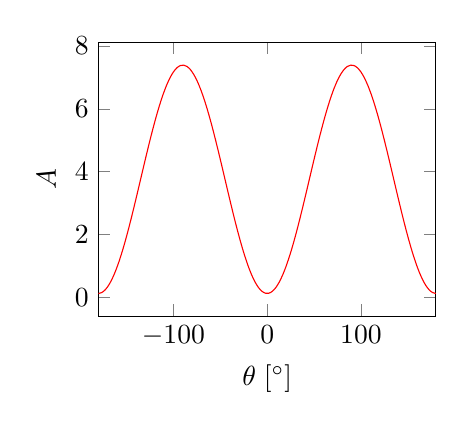
\begin{tikzpicture}
					\begin{axis}[
						height=12\baselineskip,
						xlabel = {$\theta \; [\si{\degree}]$},
						ylabel = {$A$},
						xmin = -180,
						xmax = 180,
					]
						\addplot [
							domain = -180:180,
							samples=100,
							color=red,
							smooth,
						] {exp(-2)*(cos(x))^2 + exp(2)*(sin(x))^2};
				\end{axis}
				\end{tikzpicture}
				\caption{グラフの例}\label{fig:ラベル}
			\end{figure}

			\plotcsv{csvのプロット}{
				xlabel={$x$},
				ylabel={ランダムな値},
			}{
				x index=0,
				y index=1,
			}{../fig_README/random_data.csv}

			\begin{figure}[H]
				\centering
				\begin{tikzpicture}
					\begin{axis}[
						height=13\baselineskip,
						width=0.8\columnwidth,
						xlabel={乱数1},
						ylabel={乱数2},
						legend pos=south east,
						grid=major,
						xtick distance=0.2,
						ytick distance=0.2,
						minor x tick num=4,
						minor y tick num=4,
					]
						\addplot table [
							x index=0,
							y index=1,
							only marks,
							mark=circle,
						] {../fig_README/random_data.csv};
						\addlegendentry{測定点}
						\addplot [
							domain=0:1,
							samples=100,
							color=red,
							smooth,
						] {x^2};
						\addlegendentry{理論線など}
					\end{axis}
				\end{tikzpicture}
				\caption{凡例付き}
			\end{figure}

			\begin{figure}[H]
				\centering
				\begin{tikzpicture}
					\begin{axis}[
						height=13\baselineskip,
						width=0.8\columnwidth,
						xlabel={乱数2},
						ylabel={乱数1},
						ymax = 1,
						ymin = 0,
						legend style={
							at={(1,0.5)},
							anchor=east,
						},
					]
						\addplot table [
							x index=1,
							y index=0,
							only marks,
							mark=circle,
						] {../fig_README/random_data.csv};
						\addlegendentry{$rand$}
					\end{axis}
				\end{tikzpicture}
				\caption{凡例の位置の調整}
			\end{figure}

		\sct{2}{表}
			\begin{table}[H]
				\centering
				\caption{表の例}
				\begin{tabular}{l|c}
					\hline
					原因 & 割合\\
					\hline
					A & \SI{4}{\percent}\\
					B & \SI{5}{\percent}\\
					C & \SI{2}{\percent}\\
					D & \SI{3}{\percent}\\
					E & \SI{1}{\percent}\\
					\hline
					計 & \SI{15}{\percent}\\
					\hline
				\end{tabular}
			\end{table}

		\sct{2}{リスト}
			enumitemパッケージを読み込んでいる前提。
			leftmargin=*をつけることで、左端が前後の文章と合う。
			インデントしたい場合は適切な値を入れる。\\
			参照\url{https://konoyonohana.blog.fc2.com/blog-entry-58.html}
			\begin{enumerate}[label={第\arabic*章}, leftmargin=*]
				\item aaa\\
					aaaについて
				\item bbb\\
					bbbについて
			\end{enumerate}
			leftmargin=0ptではラベル部分は左に飛び出し、テキスト部分の左が左端に合う。
			\begin{enumerate}[label={\arabic*.}, leftmargin=0pt]
				\item aaa\\
					aaaについて
				\item bbb\\
					bbbについて
			\end{enumerate}
			全角一文字分インデントしたい場合は、leftmargin=*, labelindent=1zwとする。
			\begin{enumerate}[leftmargin=*, labelindent=1zw]
				\item aaa\\
					aaaについて
				\item bbb\\
					bbbについて
			\end{enumerate}

	\sct{1}{siunitx}
		ここにある以外にも\tbs numlist, \tbs numrange, \tbs qtylistなどがある\url{http://www.yamamo10.jp/yamamoto/comp/latex/make_doc/unit/index.php}\\
		単位のみの出力では\tbs siと\tbs unitが、単位と数字では\tbs SIと\tbs qtyが使えるが, \tbs si, \tbs SIは古いバージョンとの互換性のために残されているだけで, \tbs unit, \tbs qtyを使った方がいいらしい\url{https://tex.stackexchange.com/questions/603217/should-i-use-qty-or-si-for-siunitx}。
		ただしphysicsパッケージと\tbs qtyコマンドが被っているため、physicsパッケージを使う場合は工夫が必要である。
		\begin{itemize}
			\item 単位付きの数字\qty{100}{\percent}
			\item 誤差と単位付きの数字\qty{3.95+-0.05}{\decibel}, \qty{2.23\pm 0.04}{s}
			\item 単位のみ\unit{\micro s}
			\item 数字のみ\num{2.232e4}
			\item 角度\ang{90}, \ang{12.3456}\\
					度分秒で表記したい場合\ang{12;34;56}などとする。\url{https://uec.medit.link/latex/ang.html}
			\item ミリとメートルの違い。ミリメートルだと間が無く、メートルメートル(そんなものは無いが)では間が空く。mの文字自体には違いは無さそう。因みに平方メートルは\si{m^2}と書く\\
					ミリメートルと判定されるもの : \unit{mm}, \unit{\milli\meter}, \unit{\milli m}, \unit{m\meter}\\
					メートルメートルと判定されるもの : \unit{\meter\meter}, \unit{m.m}
		\end{itemize}

	\sct{1}{脚注、参照}
		脚注は\tbs footnoteを使う\footnote{脚注の例}。
		同じ脚注を複数箇所に付けたい場合は\footnote{複数箇所につける脚注\label{fot:複数箇所につける脚注}}とラベルを入れておけば\tbs footrefで参照できる\footref{fot:複数箇所につける脚注}。
		脚注でbackrefしたい場合は, footnotebackrefパッケージを読み込めば良い\footnote{このテンプレートでは読み込んでいない}。

	\sct{1}{HyperSnips}

	\sct{1}{雑多メモ}
		\begin{enumerate}
			\item \warn{クォーテーション、ダブルクォーテーションは'や"を使うのではなく、バッククォート`とクォーテーション'やバッククォート2個``とクォーテーション2個''で表す。}記号の向き(?)が変わる。\\
					'クォーテーションで囲う'\\
					`バッククォートとクォーテーション'\\
					"ダブルクォーテーションで囲う"、''クォーテーション2個で囲う''\\
					``バッククォート2個とクォーテーション2個''
			\item \LaTeX で使える長さの単位\\
					\tbs baselineskip : 行の高さ, \tbs columnwidth : 一行の長さ\footnote{恐らく、2段組みでは1段の行の長さに対応する。\tbs linewidthは2段組みでは2段合わせた長さに対応する。}\\
					\href{https://ja.overleaf.com/learn/latex/Lengths_in_LaTeX}{"Lengths in LaTeX". Overleaf}
			\item \tbs mathrel\{\}\tbs middle$|$\tbs mathrel\{\} : 集合の区切り
					\begin{equation}
						\ab\{x\in \mathbb{C} \mathrel{}\middle|\mathrel{} e^{i\gamma x^3} = 1\}
					\end{equation}
			\item コマンドの引数に特殊な括弧を使うのはlatexdiffとの相性が悪いかもしれない\\
					\tbs fig\{キャプション\}\{画像パス\}(includegraphicsのオプション)\\
					としていたところ「includegraphicsのオプション」部分に\tbs DIFaddbeginや\tbs DIFaddendが入り、コンパイルエラーを吐いた。\\
					現在は\tbs fig\{キャプション\}[includegraphicsのオプション]\{画像パス\}とすることで対処している。\\
					physics2のab.braketでは\tbs ket$\left|0\right\rangle$ などと表記するので章\ref{s_sec:GitHubを用いたバックアップ:pre-commitについて}を導入しても動かない可能性がある。
			\item \tbs chapter*\{章の名前\tbs markboth\{章の名前\}\{\}\} 章を付けずにタイトル表示する。\\
					\tbs addcontentsline\{toc\}\{chapter\}\{章の名前\} 章立てせずに目次に追加するおまじない\\
					\tbs def\tbs chaptername\{章の名前\} ラベル用にchapternameを定義しておく。\\
					\tbs markbothはヘッダー左上に表示される文字を指定している。これをしない場合、ヘッダに章番号がついてしまう。
			\item \tbs zexternaldocumentで読み込んでも「参照先が見つからない」というエラーが出る場合は.tex\_intermediatesを一度消すとよい。\\
					また、存在しないファイルを指定しても特にエラーを吐いたりしないため、注意が必要である\footnote{sotsuron.texでまとめたものではそもそも同一texファイル内にlabelとrefがある判定になるため、最終的な論文には問題ないはず。}。
		\end{enumerate}


\sct{0}{\LaTeX の環境構築}[LaTeXの環境構築]
	環境構築、維持の難易度として2段階に分ける

	\sct{1}{VSCodeで\LaTeX を書けるようにする最小構成}[VSCodeでLaTeXを書けるようにする最小構成]
		\begin{enumerate}
			\item VSCode, TexLiveのインストール $\leftarrow$ 調べる\\
					TexLiveのインストールは時間がかかる
			\item VSCodeを開き、拡張機能をインストールする
					\begin{itemize}
						\item LaTeX Workshop : LaTeX書くなら必須
						\item Japanese Language Pack for Visual Studio Code : 設定画面を日本語にする
					\end{itemize}
			\item uplatexでコンパイルするための設定を行う。\\
					\url{https://qiita.com/t_kemmochi/items/dd38bbf2b823c770d1ec}\\
					を参考に「VS Code内でプレビューする場合の設定」までを行う。\\
					但し「手順4. VS Code のその他の設定」で「latex-workshop.latex.recipe.default」は「lastUsed」にする。\\
					また「latex-workshop.latex.autoClean.run」は「never」にする。
			\item 初回コンパイル時はVSCodeの画面左の\TeX $\to$ \LaTeX プロジェクトをビルド $\to$ レシピ:latexmk (uplatex) と操作する。\label{コンパイル手順}
			\item 以降は\TeX ファイルを保存すると自動でコンパイルされる。
			\item VSCodeを一度閉じた場合\ref{コンパイル手順}の手順が必要になることがある。
		\end{enumerate}

		\sct{2}{bibファイルについて}
			../bib/refs.bibにbibファイルを置く。\\
			日本語の人名では\\
			``langid = \{japanese\}''\\
			を追加する。\\
			Zoteroを使っている場合、「言語」の欄に``ja''や``japanese''と書いておけば自動で追加される。

	\sct{1}{\LaTeX を高速にコンパイルできる環境の構成}[LaTeXを高速にコンパイルできる環境を作る]
		第\ref{sec:LaTeXの環境構築:VSCodeでLaTeXを書けるようにする最小構成}章の設定から以下の変更を加える。
		\begin{enumerate}
			\item VSCodeを開き、拡張機能をインストールする\\
					以下は必須ではないがオススメのもの
					\begin{itemize}
						\item Path Intellisense : ファイルパスを書くときに補完してくれる。(しない場合は"を先頭に書いてからやるといい)
						\item HyperSnips : 正規表現でスニペットを作れる。自動変換もできる。このフォルダではhのあとにa-Z0-9のどれかを打つと\tbs hat\{a-Z0-9\}となるなど。
					\end{itemize}
			\item VSCodeの設定を開き、``ユーザー''タブで``Latex-workshop \textgreater Latex: Recipes''を調べる。\\
					``settings.jsonで編集''を選び、setting.jsonに以下を書く。\\
					/PATH/TO/LATEXMKRC/の部分は各々のファイルの場所に合せて変更する。
					% gobble=12で左のスペース12個分を無視
					% 最初に\lstset{tabsize=2}としているので、タブ1個=スペース2個でカウントされる。
					\begin{lstlisting}[gobble=12]
						"latex-workshop.latex.recipes": [
							{
								"name": "latexmk_fast",
								"tools": ["latexmk_fast"]
							},
							... // 省略
						],
						"latex-workshop.latex.tools": [
							{
								"name": "latexmk_fast",
								"command": "latexmk",
								"args": [
									"-r", "/PATH/TO/LATEXMKRC/.my_latexmkrc",
									"-g", // 変更が無くてもコンパイルを実行
									"-time", // 実行時間を表示
									"%DOC%"
								]
							},
							... // 省略
						]
					\end{lstlisting}
			\item コンパイルでエラーが出た場合はその\TeX ファイルがあるフォルダーの.tex\_intermediatesを消してから\ref{コンパイル手順}をしてみる
		\end{enumerate}

\sct{0}{GitHubを用いたバックアップ}
	\href{https://github.co.jp/}{GitHub}はプログラミング界隈では広く使われているサイト。
	変更履歴などを残してクラウドにバックアップを取れる。
	適宜過去の変更地点に戻ることもできるため、``aaa\_v1.tex''や``aaa\_final(最後) v2.tex''などしなくてよい。
	VSCodeと同じくMicrosoftが管理しているので相性がいい。
	極稀にサイトが落ちるので注意。
	落ちてもローカルにデータは全てあるのでPC間の同期ができないこと以外に問題はない。
	以降はバックアップの方法について説明するが、読みにくいので適宜調べてほしい。

	\sct{1}{GitHubとの連携をする}
		\begin{enumerate}
			\item GitHubにアカウントを作成
			\item Gitをインストールする
			\item GitHubで新しいrepositoryを作る\\
					\href{https://github.co.jp/}{GitHub}で左上の緑の``New''ボタンを押す
			\item Repository nameはフォルダーと同じイメージ
			\item {\Large\textcolor{red}{Privateを選ぶ}}\\
					public(デフォルト)のままだと全世界に公開してしまう
			\item ほかはデフォルトで右下の``Create repository''
			\item GitHub上での操作は一旦終わり
			\item このフォルダーをPCの適当なフォルダーにコピーする
			\item VSCodeを開く
			\item ``フォルダーを開く''でコピーしたフォルダーを開く
			\item VSCodeの左、上から3番目の丸が線で繋がったマークを押す
			\item ``リポジトリを初期化''
			\item ``ソース管理''の部分にカーソルをあわせ、右端に表示された``$\cdots$''を選ぶ
			\item ``リモート'' $\to$ ``リモートの追加''
			\item ログインする\\
					ここのログイン方法が稀に変化するため、調べる
			\item 先ほど作ったリポジトリを選ぶ
			\item ``変更''の部分にカーソルをあわせ、右端に表示された``+''を選ぶ
			\item ``✓コミット''の上の``メッセージ''にinitなどと入力する\\
					この欄はあとで変更履歴を見るとき、その履歴の名前となる
			\item ``✓コミット''またはCtrl+Enterでコミット
			\item ``Branchの発行''
			\item GitHubにアクセスしたら更新されているはず
		\end{enumerate}

	\sct{1}{変更履歴の保存方法}
		\begin{enumerate}
			\item VSCodeの左、上から3番目の丸が線で繋がったマークを押す\label{VSCodeソース管理}
			\item 他のPCで変更を行った場合、編集する前に``変更の同期''を行い、ローカルのファイルを最新版にする
			\item ``変更''の部分にカーソルをあわせ、右端に表示された``+''を選ぶ
			\item ``✓コミット''の上の``メッセージ''にinitなどと入力する\\
					この欄はあとで変更履歴を見るとき、その履歴の名前となる
			\item ``✓コミット''またはCtrl+Enterでコミット
			\item ``変更の同期''
		\end{enumerate}
		これを変更履歴を保存したいタイミングでする。
		多めにしておくと良い。
		研究室のPCと自分のPCの両方で論文を書く場合、変更履歴が衝突しないようにする必要がある。
		例えば、自分のPCで編集したが``変更の同期''をする前に、研究室のPCで編集して``変更の同期''を行った場合、Gitはクラウドと自分のPCのファイルのどちらが新しいか分からなくなり、面倒なことになる。
		したがって、編集するPCを変える前に``変更の同期''をしておく必要がある。
		\warn{つまり、研究室から帰るときに``変更の同期''をしておくのがよい。}

	\sct{1}{タグ}
		Git タグを使うことで「歴史上の重要なポイントに印をつけることができます」\url{https://git-scm.com/book/ja/v2/Git-%E3%81%AE%E5%9F%BA%E6%9C%AC-%E3%82%BF%E3%82%B0}
		つまり、特定のコミットに印を付け、素早くアクセスできるようになる。
		先生に提出した時やそのコメントを反映した時など、ある区切りがついたコミットにつけておくと編集履歴の管理やバックアップの意味で便利である。

		タグの作成手順
		\begin{enumerate}
			\item VSCodeの左、上から3番目の丸が線で繋がったマークを押す
			\item ↓ソース管理の右端に・・・があるのでクリック
			\item タグからタグの作成
			\item コマンドラインで``git push origin タグ名''をする
		\end{enumerate}

	\sct{1}{pre-commitについて}
		Gitには``Git Hooks'', ``Git フック''と呼ばれる機能がある。
		これは様々なGitコマンドが実行される直前または直後に各コマンドに対応した特定のスクリプトを実行する機能である。
		``pre-commit''はcommitコマンドが実行される直前に呼び出される。
		/pre-commitファイルの中身は, latexdiffを用いて前回のコミットと今回コミットしようとしているtexファイルの差分を/diff/diff\_ファイル名.texに書き出し、それをpdfにコンパイルするというものである。
		この機能を使いたい場合は/pre-commitファイルを/.git/hooks/以下にコピーする。
		また、場合によっては``chmod u+x pre-commit''などで実行権限を付与する必要がある。
		\warn{そもそもpdfで差分を見る必要がない、コミットに掛かる時間が非常に伸びる、という点から使用は非推奨とする。}

	\sct{1}{Branchについて}
		GitにはBranchという機能がある。
		例えば、「章の構造を大きく変えたいけど、戻すかもしれないから今のバージョンも残しておきたい」というときに、ブランチを利用する。
		デフォルトでは``main''ブランチを使っている。
		これは"木"で言うところの``幹''に相等する。
		ブランチを作成すると、``枝''を作ることができ、``幹''とは別の編集履歴を紡いで行くことができる。
		大きく変える前に戻したいときはブランチを変更すると戻すことができる。
		大きく変えた後のものを``幹''にしたい場合はマージするといい。
		詳しくは各自調べてください。

	\sct{1}{GitとGitHubの違い}
		Gitはローカルでバージョン管理ができるもの。
		変更履歴を``木''として管理している。
		GitHubはGitの``木''をクラウドにも作る。

		コミットはローカルの``木''に変更履歴を追加する。
		プッシュするとGitHubのクラウド上の``木''とローカルの``木''を同期させる(語弊があるが簡単にした)。

\sct{0}{\LaTeX 以外の環境構築}[LaTeX以外の環境構築]
	\sct{1}{drawio}
		VSCodeに拡張機能の``Draw.io Integration''をインストールする。
		デフォルトだと黒背景で見ずらいので、ユーザー設定の``Hediet \textgreater Vscode-drawio: Theme''を``Kennedy''などにする。
		またpngファイル全てをdrawioで開く設定になっている(.drawio.png以外の.pngも)。
		``Workbench: Editor Associations''に項目: *.drawio.png, 値: hediet.vscode-drawioを設定する。
		項目: *.png, 値: hediet.vscode-drawioがあれば消す。

		拡張子.drawio.pngで保存すると, drawioからは編集することができ, \LaTeX からはpngファイルとしてそのまま読み込めるので非常に便利である。
		drawio.pngを使う場合、drawio上で画像サイズが小さいとPDF上で解像度が悪くなる。
		drawioのフォントサイズ40pt$\sim$50pt, 線の太さ4pt程度に合わせてA4約3ページ\warn{以上}を目安に、\warn{とにかく大きく図を書く}。

	\sct{1}{Zotero}
		アドオンの``ZotFile''と``Better BibTex for Zotero''をインストールする。

		\sct{2}{Better BibTex for Zotero}
			一つコレクションに引用するものをまとめる。
			そのコレクションを右クリック、``コレクションをエクスポート''、フォーマット:``Better BibLaTex''、``Keep updated''にチェック、bibファイルを置く場所を選択する。

			bibファイルの自動更新を切る場合はZoteroの設定から``Better BibTex''、``Open Better BibTex preferences...''、``Automatic export''、自動更新を切るbibファイルを選択、一番下の``Remove''


\sct{0}{latexmkについて}[latexmkについて]
	latexをpdfに変換する際、refやciteなどのために複数回コマンドを実行する必要がある。
	例えば, uplatex$\rightarrow$ uplatex $\rightarrow$ biblatex $\rightarrow$ uplatex $\rightarrow$ dvipdfmx など。
	しかし、この一連の流れを自分で管理するのは困難な上、texファイルの中身や編集内容によっては一部を省略することができ、余分に実行すると無駄に時間がかかる。
	そこで, latexmkを使うと必要に応じて適切なコマンドを実行してくれる。
	latexmkの設定ファイルは一般にlatexmkrcという名前が使われる。
	latexmkrcはPerlというプログラミング言語で書かれ、
	$\$latex = `uplatex';$や$\$latex =`lualatex';$
	と書いてコンパイルに使う処理系をuplatexやlualatexと指定することができる。
	このテンプレートでは``.my\_latexmkrc''というファイル名にしている。

	\sct{1}{.my\_latexmkrcについて}[.mylatexmkrcについて]
		元は\href{https://qiita.com/JyJyJcr/items/69769c88eea9d0dae152}{``ただしい高速LaTeX論''. Qiita}を参考にした。
		Windowsでも動くように改造してある。
		変更があった場合のみプリアンブルの読み込みを行うようにすることで、大半の場合でパッケージの読み込みをスキップし、大幅にコンパイル時間を短くすることができる。
		変更があったかどうかは、プリアンブルを読み込み、空の行や各行の先頭・最後の空白、コメントを無視した部分が前回のコンパイル時と比較して判定している。
		また、画像も12時間キャッシュするようにしてある\footnote{本当にキャッシュされているのかは不明。コンパイルしたときに画像が更新されないような事態は起きていないため放置している。}。

\end{document}